\documentclass{scrartcl}
%\setlength{\textwidth}{\paperwidth}
%\addtolength{\textwidth}{-3in}
%\calclayout

\usepackage{amsmath, amssymb}
\usepackage{booktabs}

\usepackage{caption}
\usepackage{subcaption}
\captionsetup[table]{justification=justified, singlelinecheck=false}

\usepackage[dvipsnames]{xcolor}
\usepackage{tikz}

\newcommand{\RRR}{
  
\begin{tikzpicture}
    \node[circle, draw, fill=Red, inner sep= 0pt, text width=1em, align=center] (n) at (0,0) {$\scriptscriptstyle R$};
  \end{tikzpicture}
}

\newcommand{\WWW}{
  
\begin{tikzpicture}
    \node[circle, draw, fill=White,  inner sep= 0pt, text width=1em, align=center] (n) at (0,0) {$\scriptscriptstyle W$};
  \end{tikzpicture}
}

\newcommand{\BBB}{
  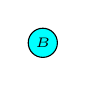
\begin{tikzpicture}
    \node[circle, draw, fill=Cyan,  inner sep= 0pt, text width=1em, align=center] (n) at (0,0) {$\scriptscriptstyle B$};
  \end{tikzpicture}
}

\newcommand{\GGG}{
  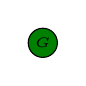
\begin{tikzpicture}
    \node[circle, draw, fill=Green,  inner sep= 0pt, text width=1em, align=center] (n) at (0,0) {$\scriptscriptstyle G$};
  \end{tikzpicture}
}

\newcommand{\YYY}{
  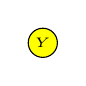
\begin{tikzpicture}
    \node[circle, draw, fill=Yellow,  inner sep= 0pt, text width=1em, align=center] (n) at (0,0) {$\scriptscriptstyle Y$};
  \end{tikzpicture}
}

\newcommand{\XXX}{
  
\begin{tikzpicture}
    \node[circle, draw, fill=Gray!40,  inner sep= 0pt, text width=1em, align=center] (n) at (0,0) {$\scriptscriptstyle X$};
  \end{tikzpicture}
}

\newcommand{\hugeskip}{\vspace{18pt}}

\newtheorem{example}{Example}
\numberwithin{example}{section}

\title{SATB}
\subtitle{A Colourful Game of Musical Puzzles}
\author{Michael Purcell}
\date{}


\begin{document}
\maketitle
\section{Introduction}\label{section:introduction}
SATB is a game for 1-5 players who work together to create a \emph{composition}.
A composition is a two-dimensional array of \emph{colours}.   
Each row of a composition is called a \emph{voice} while
each column is called a \emph{beat}.
Players create compositions by choosing which colour each voice will play on
each beat. 

\begin{figure}[ht]
\centering
\begin{subfigure}[t]{0.4\textwidth}
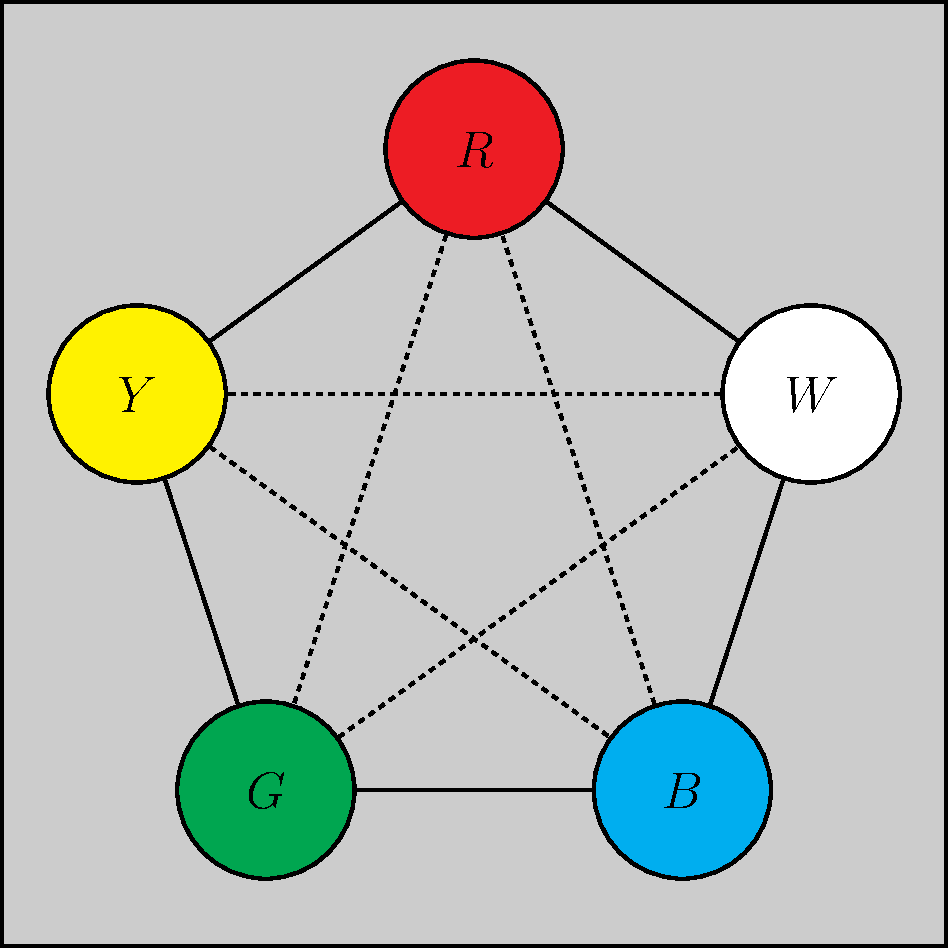
\includegraphics[width=\textwidth]{game_board.pdf}
\caption{The SATB game board.}
\end{subfigure}
\qquad
\begin{subfigure}[t]{0.4\textwidth}
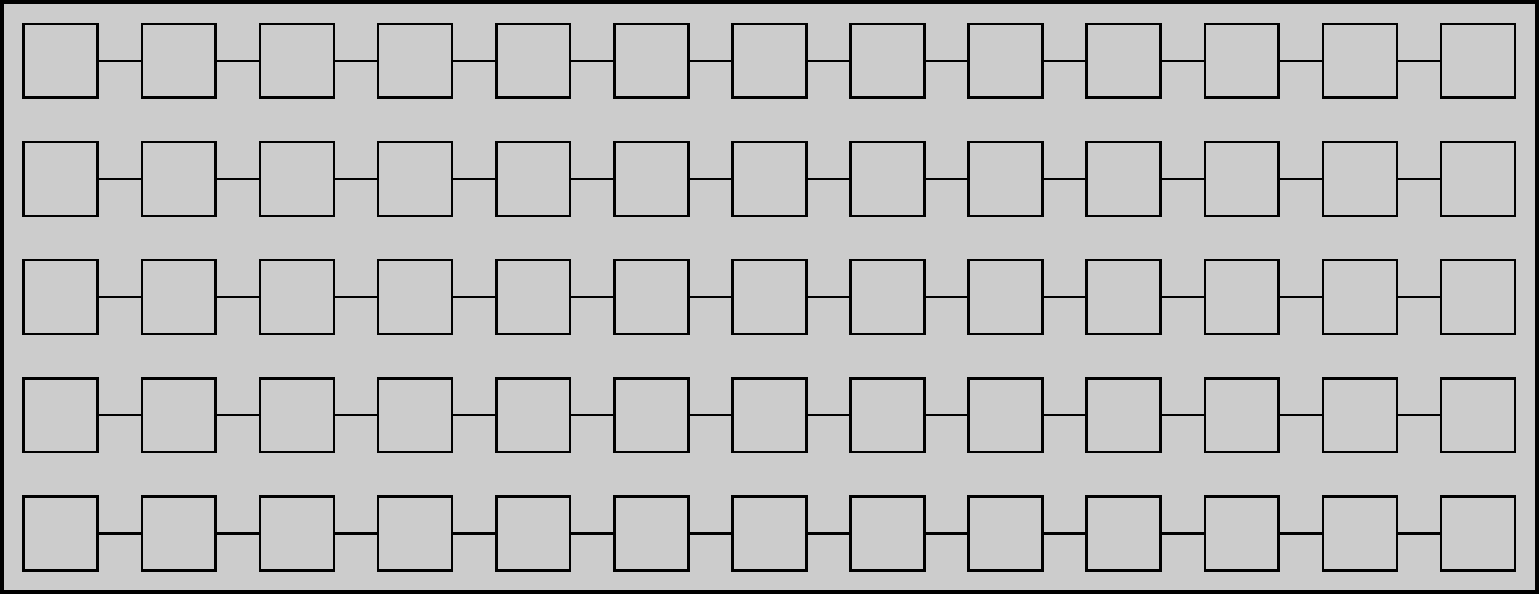
\includegraphics[width=\textwidth]{score_board.pdf}
\caption{The SATB score board.}
\end{subfigure}
\caption{Game components.}
\end{figure}

\section{Colours and Rests}
There are five colours in an SATB composition:
$\RRR$, $\WWW$, $\BBB$, $\GGG$, and $\YYY$.
We impose a structure on these five colours. This structure is depicted on the game
board by solid and dashed lines. 
If two colours are connected by a solid line then we say that they are \emph{adjacent}.
If two colours connected by a dashed line then they are not adjacent.
Given a composition $\mathbf{C} = [C_{ij}]$, we say that $i$th voice
\emph{plays a colour} on the $j$th beat if
$C_{ij} \in \begin{Bmatrix}\RRR, \WWW, \BBB, \GGG, \YYY\end{Bmatrix}$.

There is a sixth space on the game board, $\XXX$, which represents a rest.
Given a composition $\mathbf{C} = [C_{ij}]$,
we say that the $i$th voice \emph{rests} on the $j$th beat if $C_{ij} = \XXX$.


\section{Composition Rules}\label{section:composition_rules}
Each composition must satisfy a set of rules which ensure that all of the voices are
both individually interesting and mutually consistent with one another.
 
\subsection{Rhythm}
As described in the introduction, each composition is divided up into a sequence of beats. On each beat, each voice must either play a colour or rest.
Furthermore, the voices must collectively obey the \emph{continuity} rules:
\begin{description}
	\item[R1] No more than one voice may rest on each beat.
	\item[R2] No voice may rest on more than one consecutive beat.
\end{description}

\subsection{Melody}
A \emph{melody} is a sequence of colours and rests played by a single voice.  A \emph{repeat} is a when a voice plays the same colour on two consecutive beats. A \emph{step} is when a voice plays two adjacent colours on two consecutive beats. A \emph{skip} is when a voice plays two non-adjacent colours on two consecutive beats.  The direction of a step or skip
is the direction (clockwise or anticlockwise) that a token would travel on the game board
when it moves via the shortest path between the two spaces depicting the two colours involved. A melody must obey the \emph{phrasing} rules: 
\begin{description}
	\item[M1] A repeat must be followed by a step.
	\item[M2] A skip must be followed by a step in the opposite direction.
\end{description}
A \emph{phrase} is a sequence of colours that obeys the phrasing rules. Notice that a phrase may not be interrupted by a rest.
\begin{example}
There are two two-beat phrases that start with $R$:
\begin{equation}\nonumber
	\begin{bmatrix}\RRR & \WWW\end{bmatrix}
	\qquad
	\begin{bmatrix}\RRR & \YYY\end{bmatrix}
\end{equation}
and four three-beat phrases that start with $R$:
\begin{equation}\nonumber
	\begin{bmatrix}\RRR & \BBB & \WWW\end{bmatrix}
	\quad
	\begin{bmatrix}\RRR & \GGG & \YYY\end{bmatrix}
	\quad
	\begin{bmatrix}\RRR & \RRR & \YYY\end{bmatrix}
	\quad
	\begin{bmatrix}\RRR & \RRR & \WWW\end{bmatrix}
\end{equation}
\end{example}

\subsection{Harmony}
\emph{Harmony} is when several different colours are played on the same beat by different voices. A \emph{chord} is a set of colours that obey the \emph{consonance} rule:
\begin{description}
	\item[H1] No more than two colours in a chord may be adjacent.
\end{description}
A three-note chord consists of two adjacent colours and a third isolated colour. This isolated colour is called the \emph{root} of the chord.
\begin{example}
There are five one-colour chords:
\begin{equation}\nonumber
\begin{Bmatrix}\RRR\end{Bmatrix}
\qquad
\begin{Bmatrix}\WWW\end{Bmatrix}
\qquad
\begin{Bmatrix}\BBB\end{Bmatrix}
\qquad
\begin{Bmatrix}\GGG\end{Bmatrix}
\qquad
\begin{Bmatrix}\YYY\end{Bmatrix}
\end{equation}
ten two-colour chords:
\begin{equation}\nonumber
\begin{Bmatrix}
\RRR \\ \WWW
\end{Bmatrix}
\quad
\begin{Bmatrix}
\WWW \\ \BBB
\end{Bmatrix}
\quad
\begin{Bmatrix}
\BBB \\ \GGG
\end{Bmatrix}
\quad
\begin{Bmatrix}
\GGG \\ \YYY
\end{Bmatrix}
\quad
\begin{Bmatrix}
\YYY \\ \RRR
\end{Bmatrix}
\quad
\begin{Bmatrix}
\RRR \\ \BBB
\end{Bmatrix}
\quad
\begin{Bmatrix}
\WWW \\ \GGG
\end{Bmatrix}
\quad
\begin{Bmatrix}
\BBB \\ \YYY
\end{Bmatrix}
\quad
\begin{Bmatrix}
\RRR \\ \GGG
\end{Bmatrix}
\quad
\begin{Bmatrix}
\WWW \\ \YYY
\end{Bmatrix}
\end{equation}
and five three-colour chords:
\begin{equation}\nonumber
\begin{Bmatrix}
\RRR \\ \GGG \\ \BBB
\end{Bmatrix}
\qquad
\begin{Bmatrix}
\WWW \\ \YYY \\ \GGG
\end{Bmatrix}
\qquad
\begin{Bmatrix}
\BBB \\ \YYY \\ \RRR
\end{Bmatrix}
\qquad
\begin{Bmatrix}
\GGG \\ \RRR \\ \WWW
\end{Bmatrix}
\qquad
\begin{Bmatrix}
\YYY \\ \WWW \\ \BBB
\end{Bmatrix}
\end{equation}
\end{example}

\subsection{Counterpoint}
\emph{Counterpoint} is when several voices play simultaneously.
A pair of voices move in \emph{similar motion} if they both step or skip in the same direction.
A pair of voices move in \emph{contrary motion} if they step or skip in opposite directions. 
A pair of voices move in \emph{oblique motion} if one voice repeats a colour while the other voice changes colours. 
A pair of voices move in \emph{parallel motion} if they play the same colours for two consecutive beats.

A group of melodies played in counterpoint must satisfy the \emph{voice leading} rules:
\begin{description}
	\item[C1] At least one voice must move on each beat.
	\item[C2] At least one pair of voices must move in contrary or oblique motion on each beat.
	\item[C3] No pair of voices may move in parallel motion.
\end{description}

\begin{example}\label{example:valid_composition}
This composition follows the rules established above:
\begin{equation}\nonumber
\begin{bmatrix}
	\BBB & \YYY & \GGG & \WWW & \BBB \\
	\GGG & \GGG & \BBB & \GGG & \YYY \\
	\RRR & \WWW & \BBB & \WWW & \RRR
\end{bmatrix}
\end{equation}
\end{example}

\section{Game Play}
The composition rules provide criteria that can be used to evaluate a composition but do not
explain how the players create compositions during a game of SATB.  This section describes
several options for how to do so.

\subsection{Free Play}
Of course, the simplest way to play is for the players to create a composition that obeys all
of the composition rules.  This is perhaps the purest form of play but is not really a game
per se. Free play is a great way to explore the system defined by the composition rules
or to create compositions that are aesthetically pleasing.

\subsection{Figured Bass}
One embellishment that can be added to the free play version of SATB is a set of 
requirements that players' compositions must satisfy.  Unlike the composition rules
established in Section \ref{section:composition_rules}, these new requirements can change
from composition to composition.
This transforms the experience from one of unstructured play into more of a
puzzle-solving challenge.
The musical notation known as \emph{figured bass} provides one way to impose
requirements on a composition without completely specifying each voice.

In figured bass, only the \emph{bass voice} is written out explicitly.
The chords that are meant to accompany that voice are described in general terms.
Other voices then improvise melodies that are consistent with the structure that
is thereby established. 

\textcolor{red}{TODO: Describe how figured bass notation will work in SATB.}

\begin{example} 
The composition from Example \ref{example:valid_composition} is consistent with either of the the following figured bass structures:
\begin{equation}\nonumber
\begin{bmatrix}
\begin{Bmatrix} \BBB \\ \GGG \end{Bmatrix} &
\begin{Bmatrix} \GGG \\ \YYY \end{Bmatrix} &
\begin{Bmatrix} \RRR \\ \GGG \end{Bmatrix} &
\begin{Bmatrix} \YYY \\ \GGG \end{Bmatrix} &
\begin{Bmatrix} \BBB \\ \YYY \end{Bmatrix} \\ \addlinespace
\RRR & \WWW & \BBB & \WWW & \RRR
\end{bmatrix}
\begin{bmatrix}
\begin{Bmatrix} \BBB \\ \GGG \end{Bmatrix} &
\begin{Bmatrix} \GGG \\ \YYY \end{Bmatrix} &
\begin{Bmatrix} \RRR \\ \GGG \end{Bmatrix} &
\begin{Bmatrix} \RRR \\ \GGG \end{Bmatrix} &
\begin{Bmatrix} \BBB \\ \YYY \end{Bmatrix} \\ \addlinespace
\RRR & \WWW & \BBB & \WWW & \RRR
\end{bmatrix}
\end{equation}
The ambiguity is due to the fact that the bass note in the third and fourth beats is replicated
in one of the other two voices.  On beat three, the two colours that are being played are
adjacent. Therefore, the composition is consistent with only one possible chord on beat
three.  On beat four, however, the two colours that are being played are not adjacent.
Therefore, the composition is consistent with either of two possible chords on beat four.
\end{example}

\begin{table}[ht]
\caption{Generate a random figured bass structure for a composition.}
\centering
\begin{subtable}[t]{0.9\textwidth}
\centering
\caption{Generate random phrases to create a bass voice for a composition.\newline }
\begin{tabular}{@{}r l l@{}}
\toprule
Die Roll & First Move & Second Move \\
\midrule
1 & Step clockwise & - \\
2 & Step anticlockwise & - \\
3 & Repeat & Step clockwise \\
4 & Repeat & Step anticlockwise \\
5 & Skip clockwise & Step anticlockwise \\
6 & Skip anticlockwise & Step clockwise \\
\bottomrule
\end{tabular}
\end{subtable}

\bigskip\bigskip

\begin{subtable}[y]{0.9\textwidth}
\centering
\caption{Generate random chords to accompany each colour in the bass voice.\newline}
\begin{tabular}{@{}r c c c c c@{}}
\toprule
Die Roll & \multicolumn{5}{c}{Bass Voice} \\
                   \cmidrule(l{0.75em}){2-6} \addlinespace[0.25em]
             & \RRR & \WWW & \BBB & \GGG & \YYY \\
\midrule \addlinespace
$\{1,2\}$ & $\begin{Bmatrix} \BBB \\ \GGG\end{Bmatrix}$ & $\begin{Bmatrix} \GGG \\ \YYY\end{Bmatrix}$ & $\begin{Bmatrix} \YYY \\ \RRR\end{Bmatrix}$ & $\begin{Bmatrix} \RRR \\ \WWW\end{Bmatrix}$ & $\begin{Bmatrix} \WWW \\ \BBB\end{Bmatrix}$ \\[1.5em]
$\{3,4\}$ & $\begin{Bmatrix} \WWW \\ \GGG\end{Bmatrix}$ & $\begin{Bmatrix} \BBB \\ \YYY\end{Bmatrix}$ & $\begin{Bmatrix} \GGG \\ \RRR\end{Bmatrix}$ & $\begin{Bmatrix} \YYY \\ \WWW\end{Bmatrix}$ & $\begin{Bmatrix} \RRR \\ \BBB\end{Bmatrix}$ \\[1.5em]
$\{5,6\}$ & $\begin{Bmatrix} \BBB \\ \YYY\end{Bmatrix}$ & $\begin{Bmatrix} \GGG \\ \RRR\end{Bmatrix}$ & $\begin{Bmatrix} \YYY \\ \WWW\end{Bmatrix}$ & $\begin{Bmatrix} \RRR \\ \BBB\end{Bmatrix}$ & $\begin{Bmatrix} \WWW \\ \GGG\end{Bmatrix}$ \\ \addlinespace
\bottomrule
\end{tabular}
\end{subtable}
\end{table}


\end{document}
